\section{Mechanisms of Sintering}\label{sec:mechanisms}

The following elaborations on the basic theory of sintering are based on standard literature for the topic. Some notable textbooks are those of \textcite{German1996, German2014}, \textcite{Geguzin1973}, \textcite{Kang2005} and \textcite{Exner1978}.

This work concentrates on solid state sintering, which means that there are no other than solid phases present in the system (exept the surrounding atmosphere).
Liquid phase sintering, where the material partially melts to assist closing pores, shall not be regarded.
Therefore, the term sintering shall always refer to solid state sintering from here on.

Sintering in general is a process, where powder material is densified and strengthened by thermal treatment at elevated temperatures.
The process is mainly driven by reduction of the energy stored in the system microstural features, such as grain boundaries, surfaces and other crystal defects.
These features are transformed by diffusional flows of material to reach a state of lower energy.
In this process, energy is dissipated, so it is an irreversible process.

Sintering models can be distinguished in two main branches: macroscale and microscale models. 
The former regard the porous worpiece material as a continuum with variable density. 
Stresses and strains are usually modelled using visco-plastic material laws or similar while the density evolves during thermal treatment or plastic deformation (mechanical compaction). 
Numerical solution are commonly obtained by use of the \gls{FEM}.
The focus of these models usually lies in the analysis of density, strain and stress distributions, as well as damage estimation, in a component with often complex geometry.
Examples for these models are found in \textcite{Olevsky1998, Safonov2019, Kraft2004, Al-Qudsi2014, Shi2023}. 
These models will not be considered in the following, as this work concentrates on the second kind.

Microscale models regard the interaction between distinct grains resp. powder particles and the evolution of their interfaces to each other and the environment. 
The solution space typically includes from two to a limited number of distinct particles or a defined \gls{RVE}. 
Physics-based models model the distinct diffusion mechanisms occuring and their effect on the particle and/or pore shape. 

\begin{figure}
	\centering
	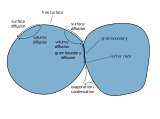
\includegraphics{img/basic_theory/diffusion_mechanisms}
	\caption{Schematic Overview of Diffusion Mechanisms Observed in Sintering Processes}
	\label{fig:introduction/state_of_the_art/diffusion_mechanisms}
\end{figure}

In common sintering processes the following diffusion mechanisms may occur, but their importance depends on powder geometry, process conditions and material properties.
The place and usual direction of their occurence is visualized in \autoref{fig:introduction/state_of_the_art/diffusion_mechanisms}.

\begin{description}
	\item[Volume Diffusion] Diffusion in the bulk material mediated by vacancies. Usually one of the slowest mechanisms and often neglegible.
	\item[Surface Diffusion] Diffusion along free surfaces (interfaces with surrounding atmosphere or vacuum). Much faster than volume diffusion.
	\item[Grain Boundary Diffusion] Diffusion along grain boundaries (solid-solid interfaces). Usually slower than surface diffusion but faster than volume diffusion.
	\item[Evaporation/Condensation] Evaporation of atoms to the gas phase and condensation at another point. Fast transport through the gas phase, but usually occurs only at very high temperatures or with very volatile substances.
\end{description}

Sintering is usually distinguished in three stages:

\begin{description}
	\item[Initial/Early Stage] Creation of initial contact. Major diffusion along surfaces to the sinter neck (triple points of surfaces and grain boundary). Rapid increase of neck size but low shrinkage.
	\item[Intermediate Stage] Porosity is still open and connected. Major diffusion along grain boundaries to the pores. Removal of substance at grain boundaries leeds to large shrinkage.
	\item[Final/Late Stage] Mainly closed porosity, gas pressure in pores may affect sintering. Still mainly grain boundary, but also volume diffusion. Slow progress in shrinkage and densification.
\end{description}


\subsubsection{Mathematical Description of Particle Surfaces and Grain Boundaries}

There are basically two ways of representing the interfaces of particles to each other or the environment: sharp and diffuse interfaces. 
Both were reported to be used in sintering simulation before.

A sharp interface means that there is a defined line were the interface is supposed to be located, on one side the one phase, on ther other side the other, without any transition.
Sharp interfaces are the most straightforward approach, as most people are used to think in that way, although in reality, interfaces have a non-zero width, typically in the scale of a few atom diameters. 
One may think about the adsorption and diffusion layer on solid surfaces or the mislalignment voids between crystallites in grain boundaries. 
However, the width of interfaces is usually much smaller then the size of particles or microscopic surface features, and can therefore be neglected.
Sharp interfaces can be described directly by the coordinates of their line string, either as a linear or non-linear spline or similar, or, by following an equality condition in the solution space (e.g. level-set method or cellular automata).
The curvature of such an interface can directly be calculated by interpolation of its coordinates, f.e. for use in \autoref{eq:stress-surface-curvature}.
Models of this type are discussed in detail in \autoref{sec:sharp-interfaces}. 

A diffuse interface means that there is a certain region of transition between the two phases.
The most common approach for that is the phase field method, where the phase present at a point is defined by the value of one or multiple auxiliary variables, whose values go smoothly between \num{0} and \num{1}.
For illustration purposes the interface is often defined at a ceratin threshold value of the phase field variables, but the model usually does not work with such, but only with the gradient of the variable.
There are no hard transitions in such models, but everything is smooth (except for the limitations of numerical discretization).
Models of this type are discussed in detail in \autoref{subsec:diffuse-interfaces}.

